\documentclass[epsfig,10pt,fullpage]{article}

\newcommand{\LabNum}{3}
\newcommand{\CommonDocsPath}{../../../common/docs}
\addtolength{\textwidth}{1.5in}
\addtolength{\oddsidemargin}{-0.75in}
\addtolength{\topmargin}{-0.75in}
\addtolength{\textheight}{1.5in}
\addtolength{\evensidemargin}{0.75in}
\setlength\parindent{0pt}
\raggedbottom

\usepackage{ae,aecompl}
\usepackage{epsfig,float,times}
\usepackage[hypcap]{caption}
\usepackage[pdftex, colorlinks]{hyperref}
\usepackage{graphicx}
\usepackage[usenames, dvipsnames]{color}
\usepackage{rotating}
\usepackage{tikz}
\usetikzlibrary{automata,positioning}
\usepackage{placeins}

\widowpenalty 10000
\clubpenalty 10000

\newcommand{\red}[1]{{\color{red}\sf{#1}}}
\newcommand{\green}[1]{{\color{green}\sf{#1}}}
\newcommand{\blue}[1]{{\color{blue}\sf{#1}}}
\definecolor{PineGreen}{rgb}{0.0, 0.47, 0.44}
\definecolor{ForestGreen}{rgb}{0.13, 0.55, 0.13}
\definecolor{Brown}{rgb}{0.59, 0.29, 0.0}

\newcommand{\UPDatePublished}{Oct 2021}
\newcommand{\versnum}{21.1} %version number quartus/AMP
\newcommand{\quartusname}{Quartus\textsuperscript{\textregistered} Prime}	
\newcommand{\UPTextBar}{For \quartusname{} \versnum{}}
\newcommand{\thisyear}{2021 } %for copyright
\newcommand{\company}{FPGAcademy.org}
\newcommand{\longteamname}{FPGAcademy.org}
\newcommand{\teamname}{FPGAcademy}
\newcommand{\website}{FPGAcademy.org}

\newcommand{\productAcronym}{AMP}
\newcommand{\productNameShort}{Monitor Program}

\newcommand{\productNameMedTM}{A Monitor Program}
\newcommand{\productNameMed}{A Monitor Program}

%\newcommand{\headerLogoFilePath}[1]{#1/FPGAcademy.png}

% listings is a package that supports encapsulating source code in LaTeX conveniently
\usepackage{listings}

\def\expandparam\lstinputlisting[#1]#2{\edef\tmp{\noexpand\lstinputlisting[#1]{#2}}\tmp}

%%%%%%%%%%%%%%%%%%%% Source Code Formatting %%%%%%%%%%%%%%%%%%%%
\definecolor{globalCommentColour}{rgb}{0.588,0.588,0.588}

%%%%%%%%%%%%%%%%%%%%%%%%%%%%%%%%%%%%%%%%%%%%%%%%%%%%
% Defining language style
% NiosII ASM
\lstdefinelanguage[NiosII]{Assembler} {
  morekeywords={add, addi, and, andhi, andi, beq, bge, bgeu, bgt, bgtu, ble,  bleu, blt, bltu, bne, br, break,
  bret, call, callr, cmpeq, cmpeqi, cmpge, cmpgei, cmpgeu, cmpgeui, cmpgt, cmpgti, cmpgtu, cmpgtui, cmple,
  cmplei, cmpleu, cmpleui, cmplt, cmplti, cmpltu, cmpltui, cmpne, cmpnei, custom, div, divu, eret, flushd,
  flushda, flushi, flushp, initd, initda, initi, jmp, jmpi, ldb, ldbio, ldbu, ldbuio, ldh, ldhio, ldhu, ldhuio,
  ldw, ldwio, mov, movhi, movi, movia, movui, mul, muli, mulxss, mulxsu, mulxuu, nextpc, nop, nor, or, orhi, ori,
  rdctl, rdprs, ret, rol, roli, ror, sll, slli, sra, srai, srl, srli, stb, stbio, sth, sthio, stw, stwio,
  sub, subi, sync, trap, wrctl, wrtcl, wrprs, xor, xori, xorhi, xori},
  morekeywords=[2]{.abort, .ABORT, .align, .app-file, .ascii, .asciz, .balign, .byte, .comm, .data, .def,
  .desc, .dim, .double, .eject, .else, .end, .endef, .endif, .equ, .equiv, .err, .extern, .file, .fill, .float,
  .global, .globl, .hword, .ident, .if, .include, .int, .irp, .irpc, .lcomm, .lflags, .line, .linkonce, .ln,
  .list, .long, .macro, .mri, .nolist, .octa, .org, .p2align, .psize, .quad, .rept, .sbttl, .scl, .section,
  .set, .short, .single, .size, .sleb128, .skip, .space, .stadb, .stabn, .stabs, .string, .symver, .tag,
  .text, .title, .type, .val, .uleb128, .word},
  morekeywords=[3]{et, bt, gp, sp, fp, ea, sstatus, ra, pc, status, estatus, bstatus, ienable, ipending, cpuid,
  exception, pteaddr, tlbacc, tlbmisc, eccinj, badaddr, config, mpubase, mpuacc},
  sensitive=t,
  alsoletter=.,
  morestring=[b]",
  morecomment=[s]{/*}{*/},
  morecomment=[l]\#,
}[keywords,comments,strings]
   
%% NOTE: morekeywords=[2] are GNU directives.
   
\definecolor{niosInstructionColour}{rgb}{0.000,0.608,0.000}
\definecolor{niosDirectiveColour}{rgb}{0.000,0.000,0.902}
\definecolor{niosSpecialRegColour}{rgb}{0.000,0.000,0.000}
\definecolor{niosStringColour}{rgb}{0.808,0.482,0.000}
   
%% NOTE: To make bold use: =\bfseries\color{<colour>}
\lstdefinestyle{defaultNiosStyle} {
  language=[NiosII]{Assembler},
  stringstyle=\color{niosStringColour},
  keywordstyle=\color{niosInstructionColour},
  keywordstyle=[2]\color{niosDirectiveColour},
  keywordstyle=[3]\itshape\color{niosSpecialRegColour}
}
%%%%%%%%%%%%%%%%%%%%%%%%%%%%%%%%%%%%%%%%%%%%%%%%%%%%

%%%%%%%%%%%%%%%%%%%%%%%%%%%%%%%%%%%%%%%%%%%%%%%%%%%%
% Defining language style
% ArmA9 ASM
\lstdefinelanguage[ArmA9]{Assembler} {
  morekeywords={ADC, ADD, ADDS, AND, ANDS, B, BAL, BEQ, BGE, BGT, BL, BLT, BIC, BKPT, BLX, BNE, BX, CDP, CLZ, CMN, CMP, EOR,
  EORS, LDC, LDM, LDR, LDRB, LDRBT, LDRH, LDRSB, LDRSH, LDRT, LSL, MCR, MLA, MOV, MOVW, MOVT, MRC, MRS, MSR, MUL, MVN, ORR, PLD,
  ROR, RSB, RSC, SBC, SMLAL, SMULL, STC, STM, STR, STRB, STRBT, STRH, STRT, SUB, SUBS, SWI, SWP, SWPB, TEQ, UMLAL,
  PUSH, POP, MOVS, RORS, LSR},
  morekeywords=[2]{.abort, .ABORT, .align, .app-file, .ascii, .asciz, .balign, .byte, .comm, .data, .def,
  .desc, .dim, .double, .eject, .else, .end, .endef, .endif, .equ, .equiv, .err, .extern, .file, .fill, .float,
  .global, .globl, .hword, .ident, .if, .include, .int, .irp, .irpc, .lcomm, .lflags, .line, .linkonce, .ln,
  .list, .long, .macro, .mri, .nolist, .octa, .org, .p2align, .psize, .quad, .rept, .sbttl, .scl, .section,
  .set, .short, .single, .size, .sleb128, .skip, .space, .stadb, .stabn, .stabs, .string, .symver, .tag,
  .text, .title, .type, .val, .vectors, .uleb128, .word},
  morekeywords=[3]{SP, PC, MIDR, CTR, TCMTR, TLBTR, MPIDR, ID_PFR0, ID_PFR1, ID_DFR0, ID_MMFR0, ID_MMFR1, ID_MMFR2,
  ID_MMFR3, ID_ISAR0, ID_ISAR1, ID_ISAR2, ID_ISAR3, ID_ISAR4, CCSIDR, CLIDR, AIDR, CSSELR, TTBR0, TTRB1, TTBR2, DACR,
  DFSR, IFSR, ADFSR, AIFSR, DFAAR, IFAR, ICIALLUIS, BPIALLIS, PAR, ICIALLU, ICIMVAU, BPIALL, DCIMVAC, DCISW, V2PCWPR,
  DCCVAC, DCCSW, DDIMVAC, DCISW, TLBALLIS, TLBIMVAIS, TLBIASIDIS, TLBIMVAAIS, TLBIALL, TLBIMVA, TLBIASID, TLBIMVAA,
  PMCR, PMCNTENSET, PMCNTENCLR, PMOVSR, PMSWINC, PMSELR, PMXEVTYPER, PMXEVCNTR, PMUSERENR, PMINTENSET, PMINTENCLR,
  PRRR, NRRR, PLEIDR, PLEASR, PLEFSR, PLEUAR, PLEPCR, VBAR, MVBAR, ISR, FCSEIDR, CONTEXTIDR, TPIDRURW, TPIDRURO, TPIDRPRW},
  sensitive=f,
  alsoletter=.,
  morestring=[b]",
  morecomment=[s]{/*}{*/},
  morecomment=[l]{//},
}[keywords,comments,strings]
   
%% NOTE: morekeywords=[2] are GNU directives.
   
\definecolor{armInstructionColour}{rgb}{0.000,0.608,0.000}
\definecolor{armDirectiveColour}{rgb}{0.000,0.000,0.902}
\definecolor{armSpecialRegColour}{rgb}{0.000,0.000,0.000}
\definecolor{armStringColour}{rgb}{0.808,0.482,0.000}
   
\lstdefinestyle{defaultArmStyle} {
  language=[ArmA9]{Assembler},
  stringstyle=\color{armStringColour},
  keywordstyle=\color{armInstructionColour},
  keywordstyle=[2]\color{armDirectiveColour},
  keywordstyle=[3]\itshape\color{armSpecialRegColour}
}
%%%%%%%%%%%%%%%%%%%%%%%%%%%%%%%%%%%%%%%%%%%%%%%%%%%%

%%%%%%%%%%%%%%%%%%%%%%%%%%%%%%%%%%%%%%%%%%%%%%%%%%%%
% Defining language style
% FPGAcademy ASM
\lstdefinelanguage{ASM}{
  morekeywords = [1]{mv, mvt, mvne, mvcc, add, sub, st, ld, and, b, bne, beq, bcc, bcs},
  morekeywords = [2]{word, define},
  keywordstyle = [1]\color{ForestGreen},
  keywordstyle = [2]\color{blue},
  sensitive = true,
  morecomment = [l]{//},
}

\lstset{
  language = ASM,
  basicstyle=\small\color{black}\ttfamily,
  commentstyle=\small\color{Brown}\itshape\ttfamily,
  showstringspaces=false,
  frame=none, %lines % boxed listings
  breaklines=true,
  breakatwhitespace=true,
  tabsize=3
}
%%%%%%%%%%%%%%%%%%%%%%%%%%%%%%%%%%%%%%%%%%%%%%%%%%%%

%%%%%%%%%%%%%%%%%%%%%%%%%%%%%%%%%%%%%%%%%%%%%%%%%%%%
% Defining language style
% Java
\definecolor{javaStringColour}{rgb}{0.808,0.482,0}
%%%%%%%%%%%%%%%%%%%%%%%%%%%%%%%%%%%%%%%%%%%%%%%%%%%%

%%%%%%%%%%%%%%%%%%%%%%%%%%%%%%%%%%%%%%%%%%%%%%%%%%%%
% Defining language style
% C
\definecolor{CStringColour}{rgb}{0.808,0.482,0}

\lstset{
  language = C,
  basicstyle=\small\color{black}\ttfamily, 
  commentstyle=\small\color{PineGreen}\itshape\ttfamily,
  keywordstyle=\small\color{blue}\bfseries\ttfamily,
  showstringspaces=false,
  frame=none, %lines % boxed listings
  breaklines=true,
  breakatwhitespace=true,
  tabsize=3
}
%%%%%%%%%%%%%%%%%%%%%%%%%%%%%%%%%%%%%%%%%%%%%%%%%%%%

%%%%%%%%%%%%%%%%%%%%%%%%%%%%%%%%%%%%%%%%%%%%%%%%%%%%
% Defining language style
% Verilog
\definecolor{verilogCommentColour}{rgb}{0.000,0.502,0.000}

\lstdefinestyle{defaultVerilogStyle} {
  language={Verilog},
  keywordstyle=\color{blue},
  commentstyle=\color{verilogCommentColour}
}
%%%%%%%%%%%%%%%%%%%%%%%%%%%%%%%%%%%%%%%%%%%%%%%%%%%%

%%%%%%%%%%%%%%%%%%%%%%%%%%%%%%%%%%%%%%%%%%%%%%%%%%%%
% Defining language style
% VHDL
\lstdefinestyle{defaultVHDLStyle} {
  language={VHDL},
  keywordstyle=\color{blue},
  commentstyle=\color{verilogCommentColour}
}
%%%%%%%%%%%%%%%%%%%%%%%%%%%%%%%%%%%%%%%%%%%%%%%%%%%%

%%%%%%%%%%%%%%%%%%%%%%%%%%%%%%%%%%%%%%%%%%%%%%%%%%%%
% Defining language style
% LaTeX
\lstdefinelanguage[LocalLaTeX]{TeX}[LaTeX]{TeX}{moretexcs={bf, it, sf, lstset},}

\lstdefinestyle{defaultLocalLatexStyle} {
  language=[LocalLatex]{TeX},
  keywordstyle=\color{blue}\bfseries,
  keywordstyle=[2]\color{blue},
  keywordstyle=[3]\color{blue}\bfseries
}
%%%%%%%%%%%%%%%%%%%%%%%%%%%%%%%%%%%%%%%%%%%%%%%%%%%%

%%%%%%%%%%%%%%%%%%%%%%%%%%%%%%%%%%%%%%%%%%%%%%%%%%%%
% Defining language style
% Default
\lstset{
  basicstyle=\small\color{black}\ttfamily,
  commentstyle=\small\color{globalCommentColour}\itshape\ttfamily,
  keywordstyle=\small\color{blue}\bfseries\ttfamily,
  showstringspaces=false,
  frame=none, %lines % boxed listings
  breaklines=true,
  breakatwhitespace=true,
  tabsize=3
}
%%%%%%%%%%%%%%%%%%%%%%%%%%%%%%%%%%%%%%%%%%%%%%%%%%%%


\hypersetup{
  pdftitle={Digital Logic Lab Exercise \LabNum},
  linkcolor=blue,
  hyperindex=true,
  pdfauthor={FPGAcademy.org},
  pdfkeywords={FPGAcademy.org, FPGAcademy, Lab, Exercise, Digital Logic},
  bookmarks,
  bookmarksopen=false,
  filecolor=blue,
  pdfstartview={FitH},
  urlcolor=blue,
  plainpages=false,
  pdfpagelabels=true,
  linkbordercolor={1 1 1} %no color for link border
}



\begin{document}

\centerline{\huge Digital Logic}
~\\
\centerline{\huge Laboratory Exercise \LabNum}
~\\
\centerline{\large Latches, Flip-flops, and Registers}
~\\

\noindent
The purpose of this exercise is to investigate latches, flip-flops, and registers.

\section*{Part I}
\addcontentsline{toc}{1}{Part I}
Intel\textsuperscript{\textregistered} FPGAs include flip-flops that are available for implementing a user's circuit. 
We will show how to make use of these flip-flops in Part IV of this exercise. But
first we will show how storage elements can be created in an FPGA without using 
its dedicated flip-flops.

Figure~\ref{fig:RSlatch} depicts a gated RS latch circuit. Two styles of Verilog code
that can be used to describe this circuit are given in Figures~\ref{fig:latch_code1}
and \ref{fig:latch_code2}.
Figure~\ref{fig:latch_code1} specifies the latch by instantiating logic gates, and 
Figure~\ref{fig:latch_code2} uses 
logic expressions to create the same circuit. If this latch is implemented
in an FPGA that has 4-input lookup tables (LUTs), then only one lookup table is needed, 
as shown in Figure~\ref{fig:RSlatch_cct}$a$. 

\begin{figure}[H]
	\begin{center}
		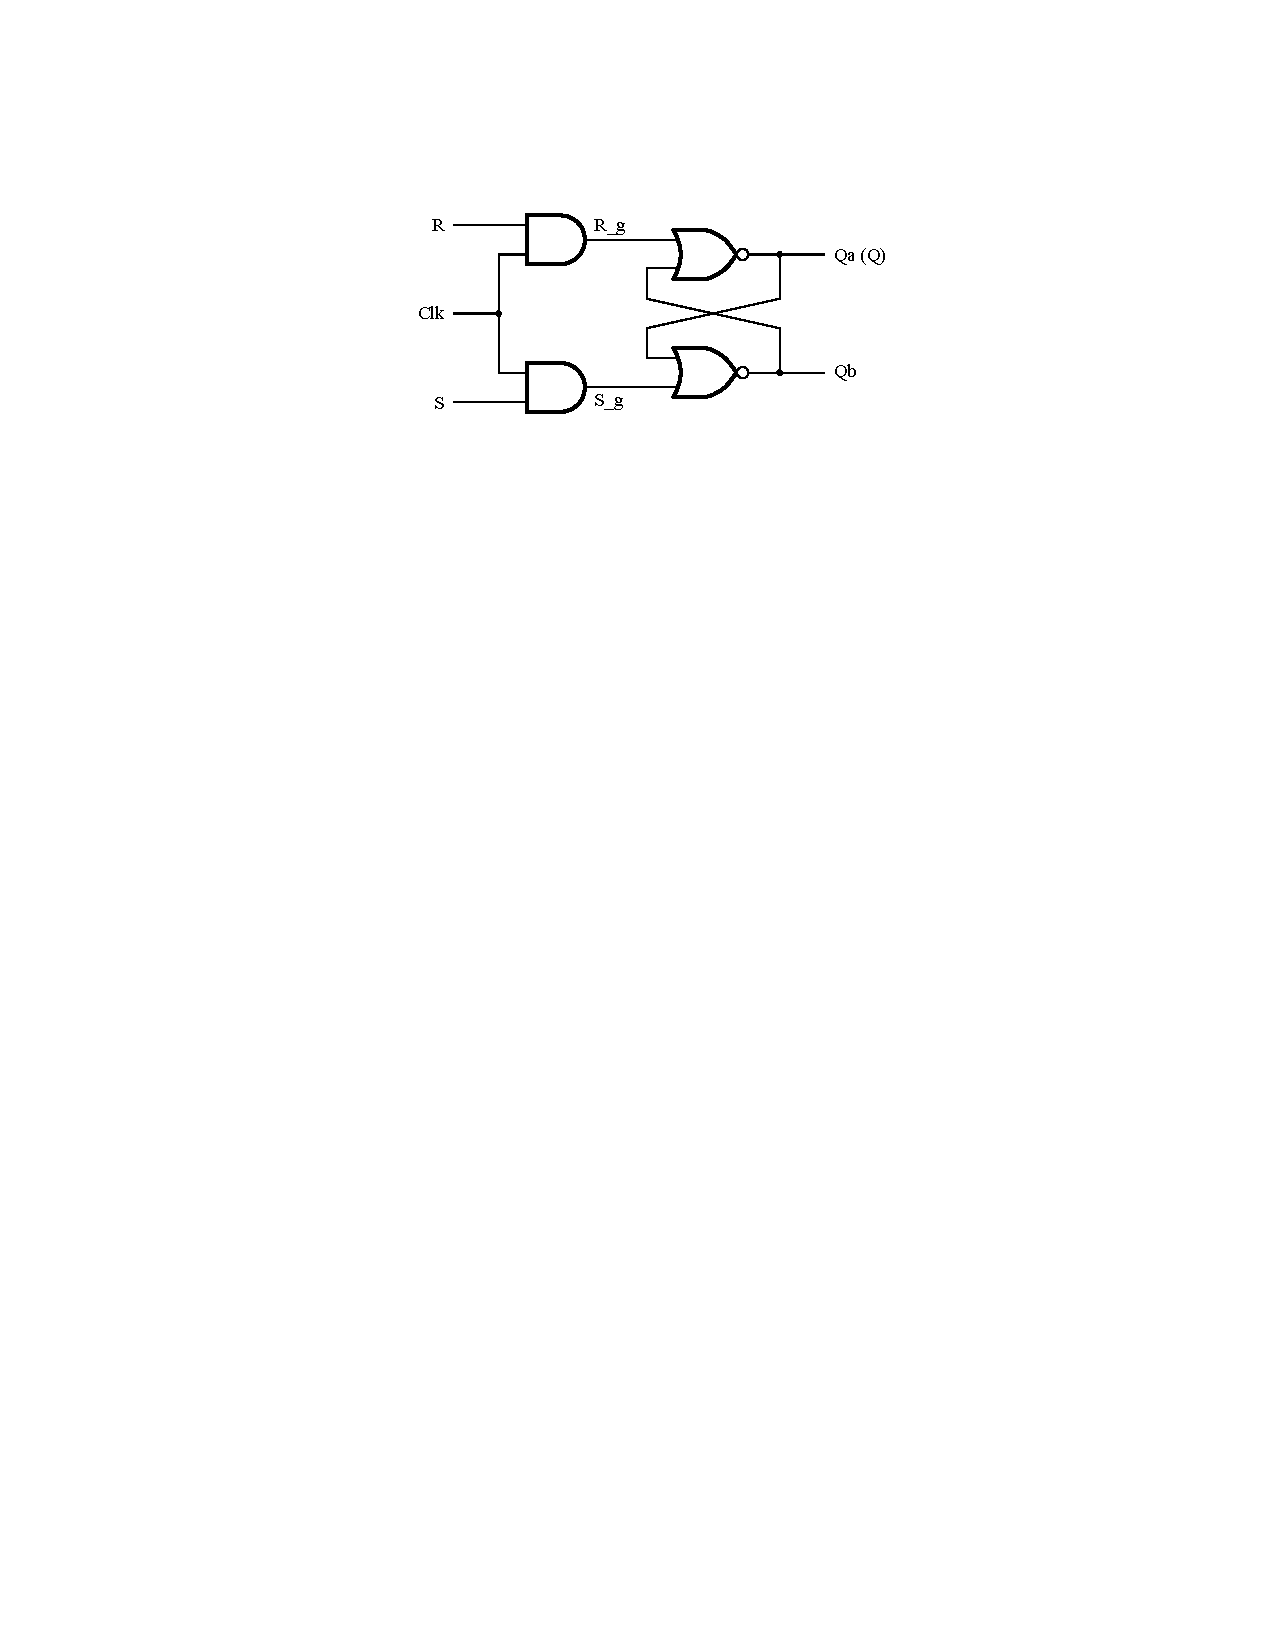
\includegraphics[]{figures/RS_latch.pdf}
	\end{center}
\caption{A gated RS latch circuit.}
\label{fig:RSlatch}
\end{figure}

\begin{figure}[H]
\begin{center}
\begin{minipage}[t]{12.5 cm}
\begin{tabbing}
ZZ\=ZZ\=ZZ\=ZZ\=ZZ\=ZZ\=ZZ\=ZZ\=ZZ\kill
// A gated RS latch \\
{\bf module} ~part1 (Clk, R, S, Q);\\
\>{\bf input} Clk, R, S;\\
\>{\bf output} Q;\\
~\\
\>{\bf wire} R\_g, S\_g, Qa, Qb /* synthesis keep */ ;\\
~\\
\>{\bf and} (R\_g, R, Clk);\\
\>{\bf and} (S\_g, S, Clk);\\
\>{\bf nor} (Qa, R\_g, Qb);\\
\>{\bf nor} (Qb, S\_g, Qa);\\
~\\
\>{\bf assign} Q = Qa;\\
~\\
{\bf endmodule}\\
\end{tabbing}
\end{minipage}
\end{center}
\caption{Specifying an RS latch by instantiating logic gates.}
\label{fig:latch_code1}
\end{figure}

\begin{figure}[H]
\begin{center}
\begin{minipage}[t]{12.5 cm}
\begin{tabbing}
ZZ\=ZZ\=ZZ\=ZZ\=ZZ\=ZZ\=ZZ\=ZZ\=ZZ\kill
// A gated RS latch\\
{\bf module} ~part1 (Clk, R, S, Q);\\
\>{\bf input} Clk, R, S;\\
\>{\bf output} Q;\\
~\\
\>{\bf wire} R\_g, S\_g, Qa, Qb /* synthesis keep */ ;\\
~\\
\>{\bf assign} R\_g = R \& Clk;\\
\>{\bf assign} S\_g = S \& Clk;\\
\>{\bf assign} Qa = $\sim$(R\_g $\mid$ Qb);\\
\>{\bf assign} Qb = $\sim$(S\_g $\mid$ Qa);\\
~\\
\>{\bf assign} Q = Qa;\\
~\\
{\bf endmodule}\\
\end{tabbing}
\end{minipage}
\end{center}
\caption{Specifying an RS latch by using Boolean expressions.}
\label{fig:latch_code2}
\end{figure}

Although the latch can be correctly realized in one 4-input LUT, this implementation
does not allow its internal signals, such as $R\_g$ and $S\_g$, to be observed, because
they are not provided as outputs from the LUT. To preserve these internal signals in 
the implemented circuit, it is necessary to include a {\it compiler
directive} in the code. In Figures~\ref{fig:latch_code1}
and \ref{fig:latch_code2} the directive /* synthesis keep */ is
included to instruct the Quartus\textsuperscript{\textregistered} compiler to use separate logic elements for each of
the signals $R\_g, S\_g, Qa,$ and $Qb$. Compiling the code produces the circuit with four
4-LUTs depicted in Figure~\ref{fig:RSlatch_cct}$b$. 

\begin{figure}[H]
	\begin{center}
		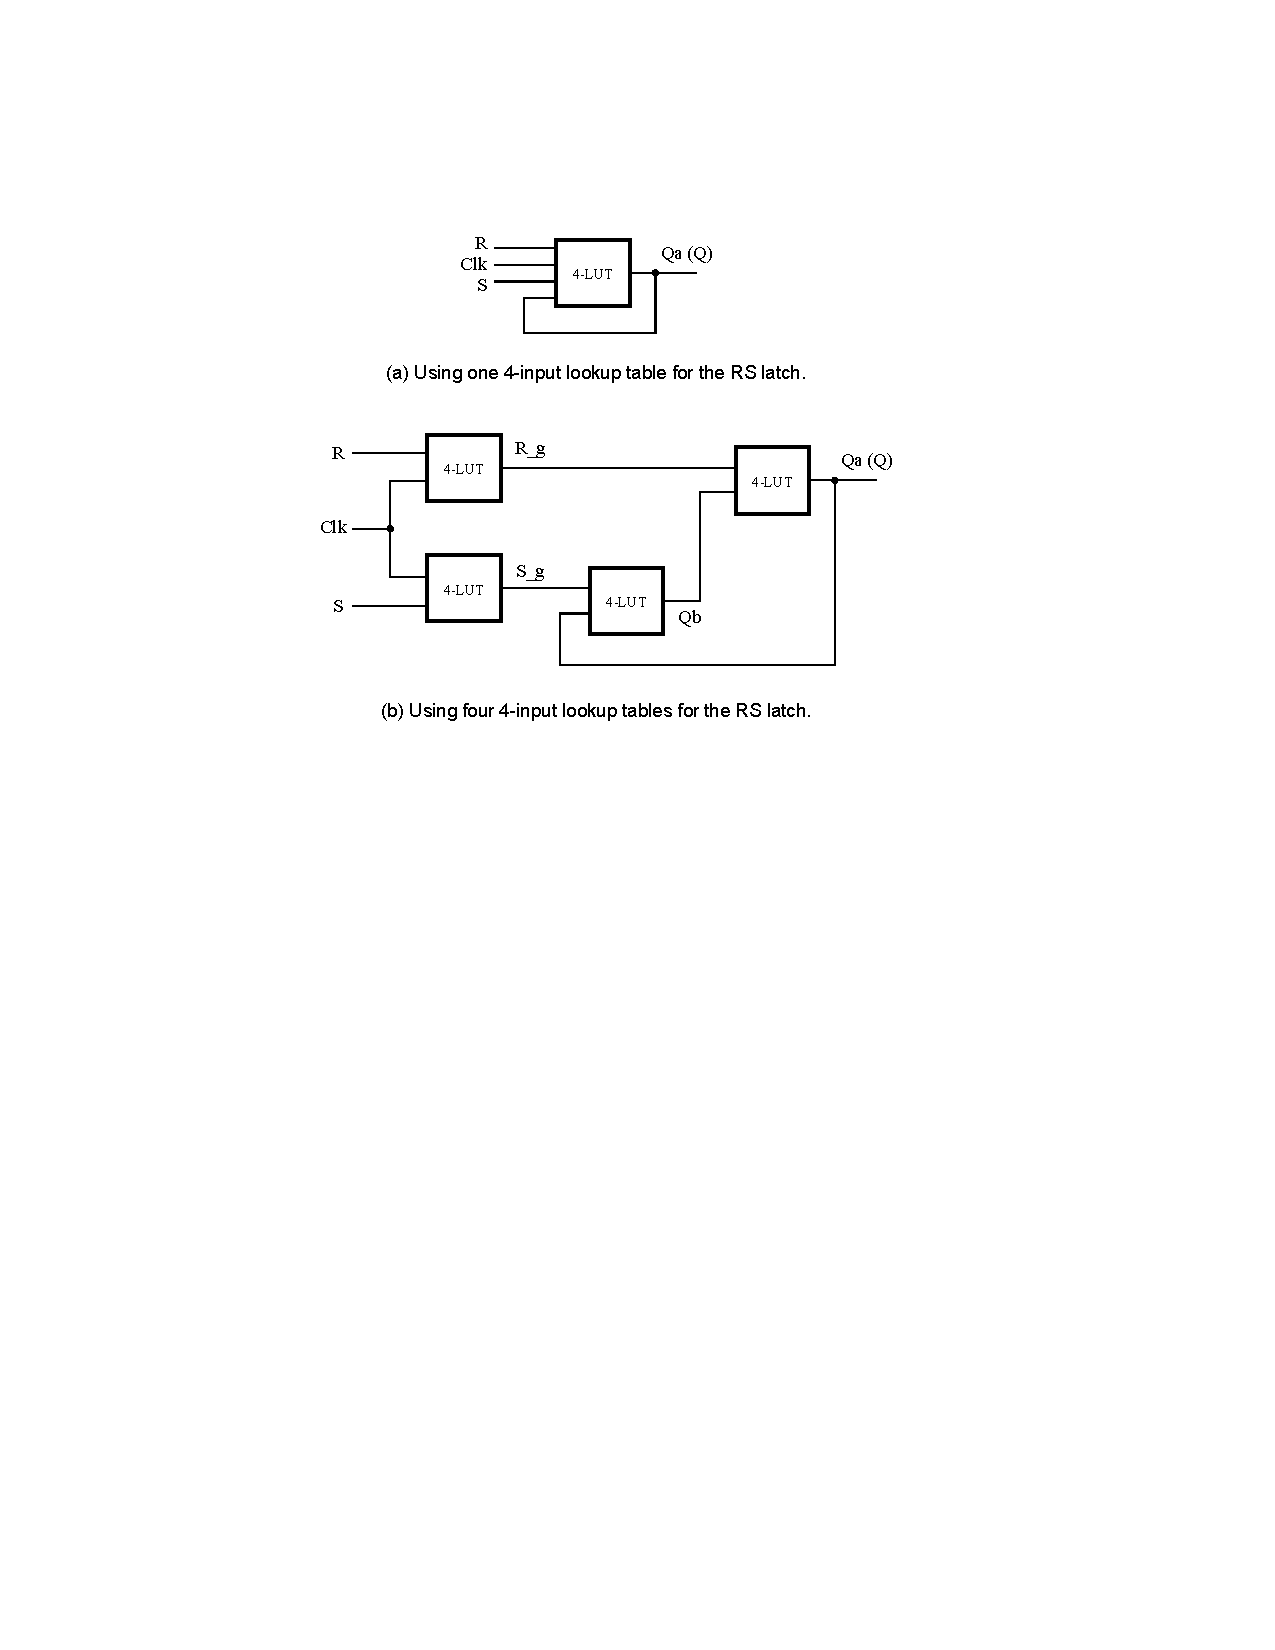
\includegraphics[]{figures/figure3.pdf}
	\end{center}
	\caption{Implementation of the RS latch from Figure~\ref{fig:RSlatch}.}
\label{fig:RSlatch_cct}
\end{figure}

Create a Quartus project for the RS latch circuit as follows:
\begin{enumerate}
\item Create a new Quartus project for your DE-series board.
\item Generate a Verilog file for the RS latch. Use the code in either Figure~\ref{fig:latch_code1} or
Figure~\ref{fig:latch_code2}
(both versions of the code should produce the same circuit) and include it in the project. 
\item Compile the code. Use the Quartus RTL Viewer tool to examine the gate-level
circuit produced from the code, and use the Technology Map Viewer tool 
to verify that the latch is implemented as shown in Figure~\ref{fig:RSlatch_cct}$b$.
\item Simulate the behavior of your Verilog code by using the simulation feature provided
in the Modelsim software. Use the testbench provided in the laboratory materials to drive
the signals for your simulation. The procedure for using Modelsim for simulation is
described in the tutorial {\it Using the ModelSim-Intel FPGA Simulator}. An example of a
vector waveform file is displayed in Figure~\ref{fig:sim}. The waveforms in the figure
begin by setting {\it Clk} $= 1$ and $R = 1$, which allows the simulation tool to
initialize all of the signals inside of the latch to known values. 
\end{enumerate}

\begin{figure}[H]
	\begin{center}
		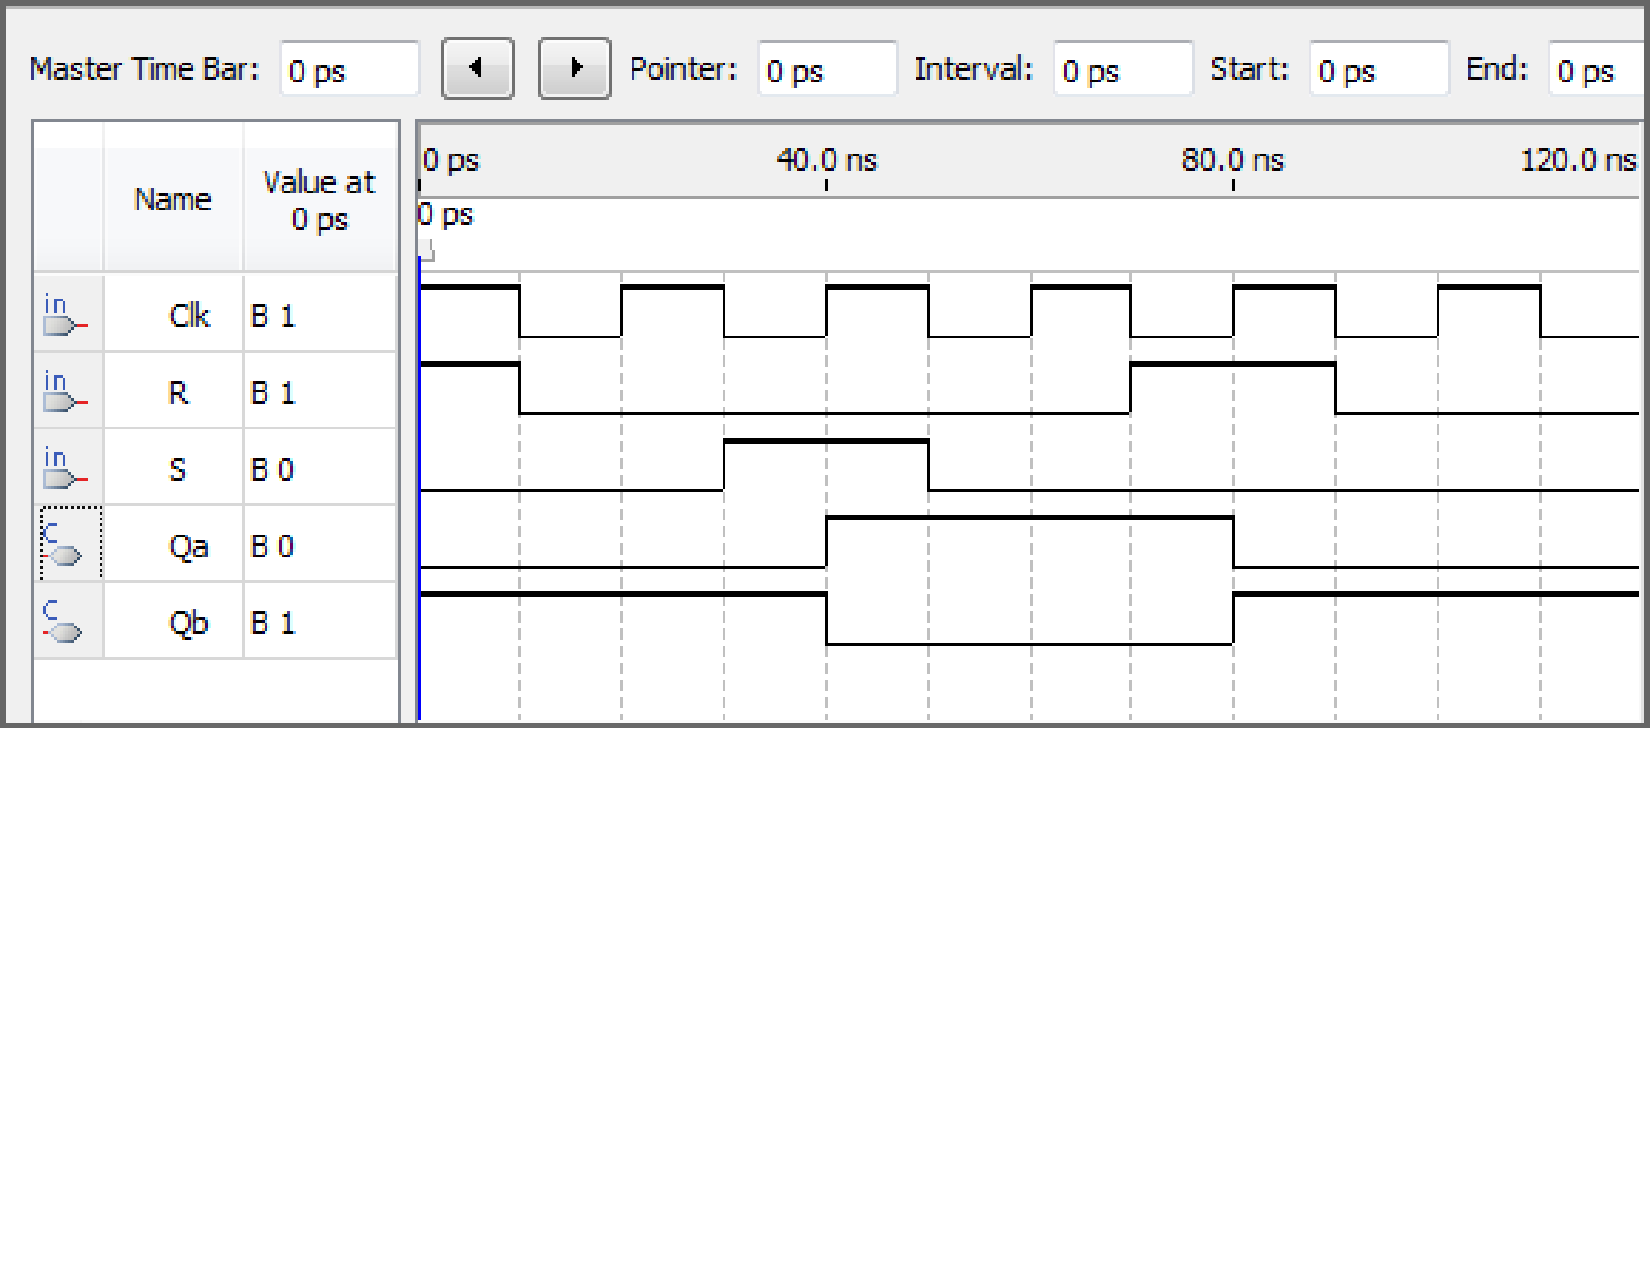
\includegraphics[width = 5in]{figures/simulation.pdf}
	\end{center}
	\caption{Simulation waveforms for the RS latch.}
\label{fig:sim}
\end{figure}

\section*{Part II}
\addcontentsline{toc}{2}{Part II}
Figure~\ref{fig:gatedD} shows the circuit for a gated D latch.
\begin{figure}[H]
	\begin{center}
		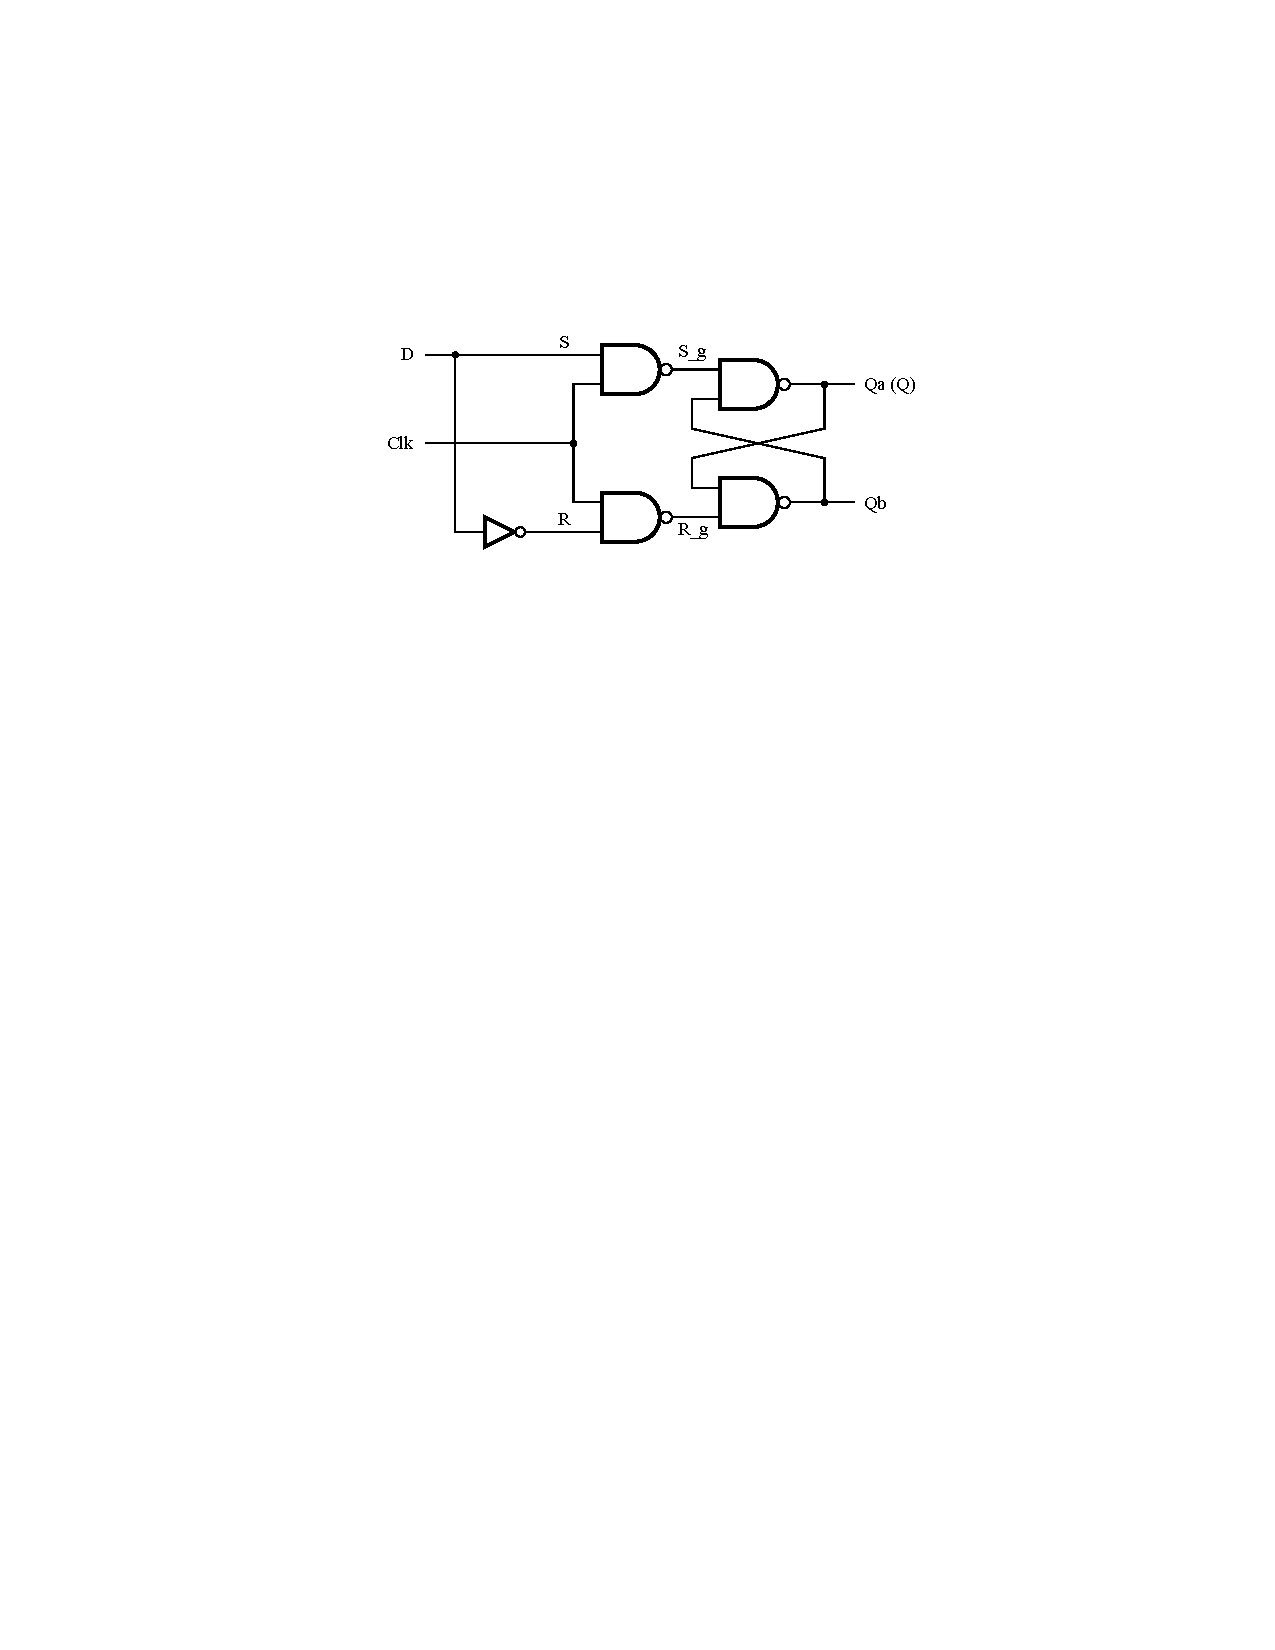
\includegraphics[]{figures/D_latch.pdf}
	\end{center}
	\caption{Circuit for a gated D latch.}
\label{fig:gatedD}
\end{figure}

Perform the following steps:
\begin{enumerate}
\item Create a new Quartus project. Generate a Verilog file using the style of code 
in Figure~\ref{fig:latch_code2} for the gated D latch. 
Use the /* synthesis keep */ directive to ensure
that separate logic elements are used to implement the signals $R, S\_g, R\_g, Qa,$ and $Qb$.
\item Compile your project and then use the 
Technology Map Viewer tool to examine the implemented circuit.
\item Verify that the latch works properly for all input conditions by using functional 
simulation. Examine the timing characteristics of the circuit by using timing simulation.
\item Create a new Quartus project which will be used for implementation of the gated D
latch on your DE-series board. This project should consist of a top-level module that 
contains the appropriate input and output ports (pins) for your board. Instantiate your
latch in this top-level module. Use switch {\it SW}$_0$ to drive the {\it D} input of the latch,
and use {\it SW}$_1$ as the {\it Clk} input. Connect the Q output to {\it LEDR}$_{0}$.
\item
Include the required pin assignments and then compile your project and download the 
compiled circuit onto your DE-series board.
\item
Test the functionality of your circuit by toggling the $D$ and {\it Clk} switches and observing 
the Q output.
\end{enumerate}

\section*{Part III}
\addcontentsline{toc}{3}{Part III}
Figure~\ref{fig:MS_FF} shows the circuit for a master-slave D flip-flop.

\begin{figure}[H]
	\begin{center}
		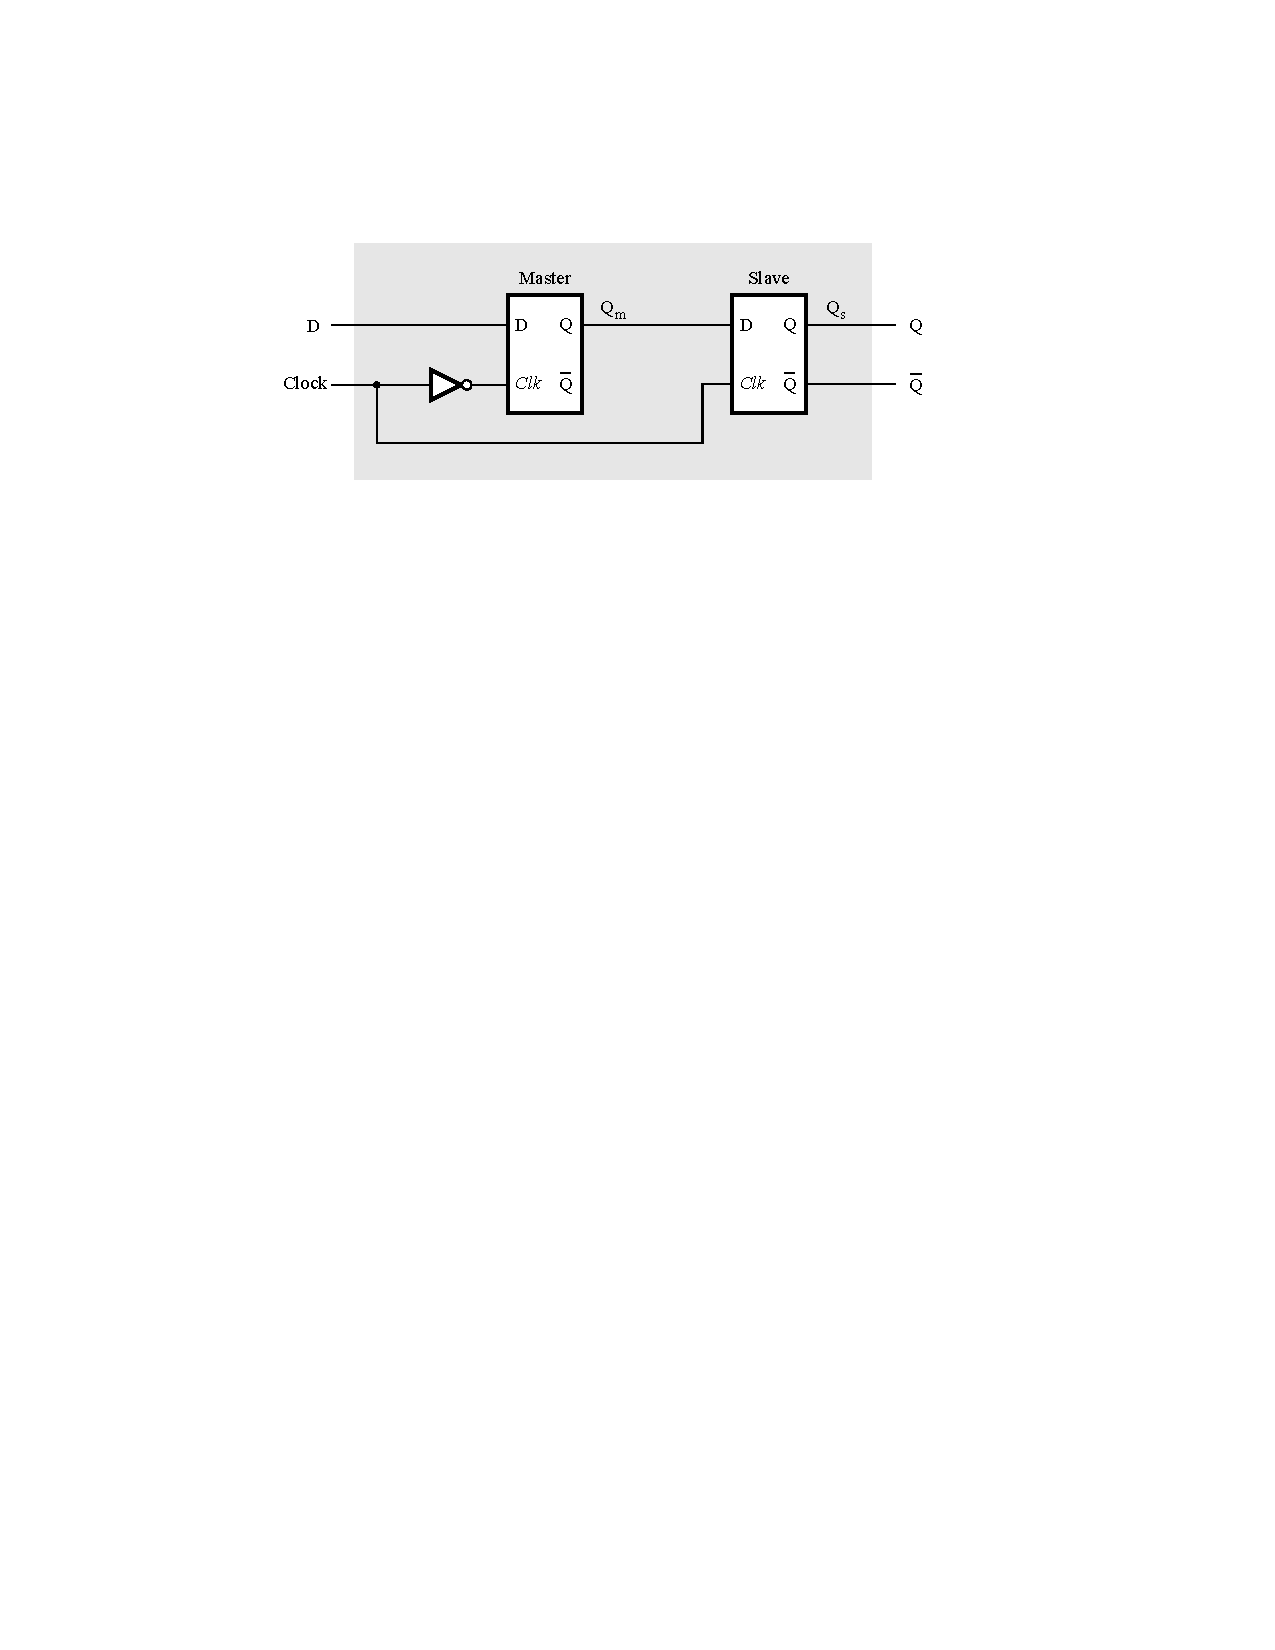
\includegraphics[]{figures/figure5.pdf}
	\end{center}
	\caption{Circuit for a master-slave D flip-flop.}
\label{fig:MS_FF}
\end{figure}

Perform the following:
\begin{enumerate}
\item Create a new Quartus project. Generate a Verilog file that instantiates two
copies of your gated D latch module from Part II to implement the master-slave flip-flop.
\item Include in your project the appropriate input and output ports for your
DE-series board. Use switch {\it SW}$_0$ to drive the D input of the flip-flop,
and use {\it SW}$_1$ as the {\it Clock} input. Connect the Q output to {\it LEDR}$_{0}$.
\item
Include the required pin assignments and then compile your project.
\item Use the Technology Map Viewer to examine the D flip-flop circuit, and use simulation to
verify its correct operation.
\item
Download the circuit onto your DE-series board and test its functionality 
by toggling the $D$ and {\it Clock} switches and observing the Q output.
\end{enumerate}

\newpage
\section*{Part IV}
\addcontentsline{toc}{4}{Part IV}
Figure~\ref{fig:waves} shows a circuit with three different storage elements: a gated D latch, 
a positive-edge triggered D flip-flop, and a negative-edge triggered D flip-flop.

\begin{figure}[H]
	\begin{center}
		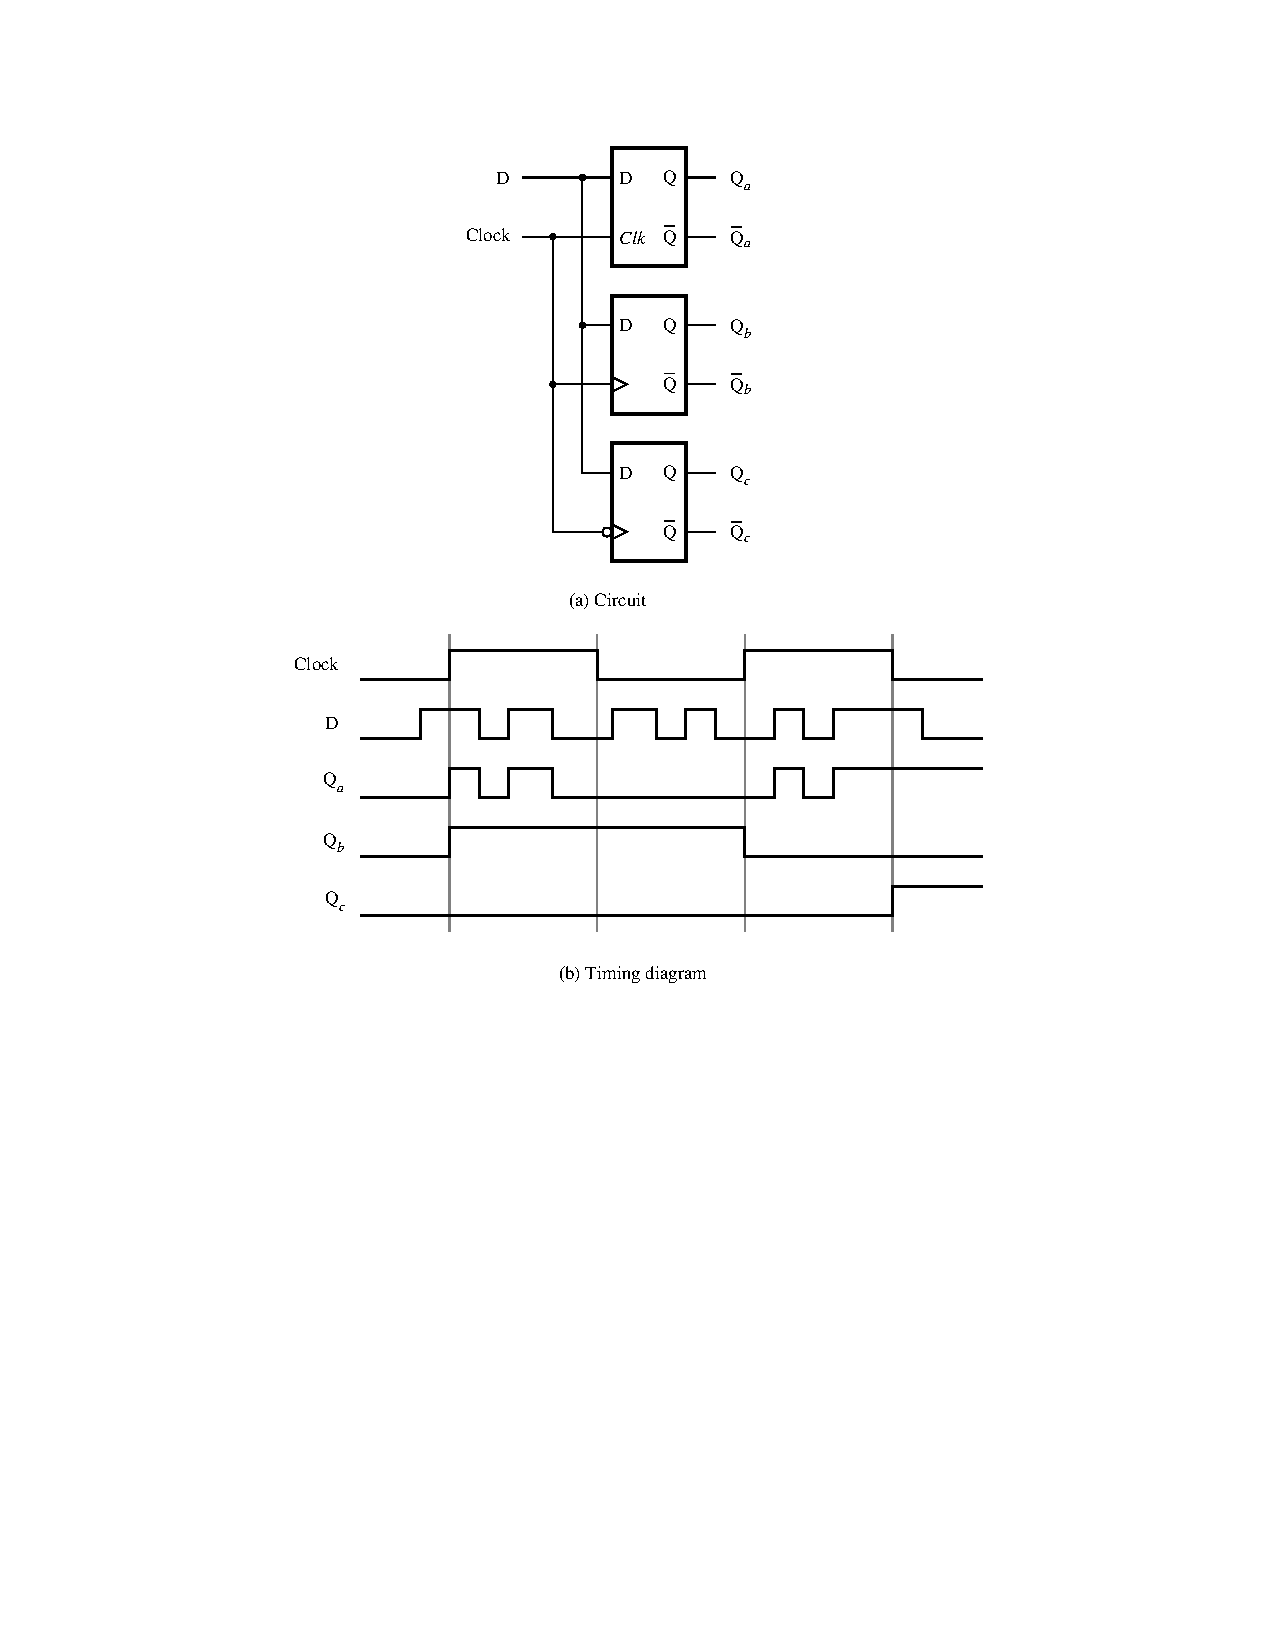
\includegraphics[]{figures/figure6.pdf}
	\end{center}
	\caption{Circuit and waveforms for Part IV.}
\label{fig:waves}
\end{figure}

Implement and simulate this circuit using the Quartus software as follows:
\begin{enumerate}
\item Create a new Quartus project. 
\item Write a Verilog file that instantiates the three storage elements. For this part you
should no longer use the /*~synthesis keep~*/ directive from Parts I to III. 
Figure~\ref{fig:behave} gives a behavioral style of Verilog code that specifies the gated D 
latch in Figure~\ref{fig:gatedD}.
This latch can be implemented in one 4-input lookup table. Use a similar style of
code to specify the flip-flops in Figure~\ref{fig:waves}.
\item Compile your code and use the Technology Map Viewer to examine the implemented circuit.
Verify that the latch uses one lookup table and that the flip-flops are implemented using
the flip-flops provided in the target FPGA.
\item Use Modelsim to simulate the circuit you created. Use the included testbench file to 
specify the inputs $D$ and {\it Clock} as indicated in Figure~\ref{fig:waves}.
Make sure that the testbench correctly instantiates the module you created and 
run the simulation to observe the different behavior of the three storage elements.
\end{enumerate}

\begin{figure}[H]
\begin{center}
\begin{minipage}[t]{12.5 cm}
\begin{tabbing}
ZZ\=ZZ\=ZZ\=ZZ\=ZZ\=ZZ\=ZZ\=ZZ\=ZZ\kill
{\bf module} D\_latch ~(D, Clk, Q);\\
\>{\bf input} D, Clk;\\
\>{\bf output reg} Q;\\
~\\
\>{\bf always} @ (D, Clk)\\
\>\>{\bf if} (Clk)\\
\>\>\>Q = D;\\
{\bf endmodule}\\
\end{tabbing}
\end{minipage}
\end{center}
\caption{A behavioral style of Verilog code that specifies a gated D latch.}
\label{fig:behave}
\end{figure}

\section*{Part V}
\addcontentsline{toc}{5}{Part V}
We wish to display the hexadecimal value of an 8-bit number $A$
on the two 7-segment displays $HEX3-2$.  We also wish to display the
hex value of an 8-bit number $B$ on the two 7-segment displays $HEX1-0$. 
The values of $A$ and $B$ are inputs to the circuit which are
provided by means of switches $SW_{7-0}$.  To input the values of $A$ and $B$, 
first set the switches to the desired value of $A$, store these switch values in a register, 
and then change the switches to the desired value of $B$.  Finally, use an adder to 
generate the arithmetic sum $S = A + B$, and display this sum on the 7-segment 
displays $HEX5-4$. Show the carry-out produced by the adder on LEDR[0].
\begin{enumerate}
\item Create a new Quartus project which will be used to implement the desired
circuit on your DE-series board.
\item Write a Verilog file that provides the necessary functionality. Use {\it KEY}$_0$ as
an active-low asynchronous reset, and use {\it KEY}$_1$ as a clock input.
\item Include the necessary pin assignments for the pushbutton switches and 7-segment
displays, and then compile the circuit.
\item Download the circuit onto your DE-series board and test its functionality 
by toggling the switches and observing the output displays.
\end{enumerate}



%%%%%%%%%%%%%%%%%%%%%%%%%%%%%%%%%%%%%%%%
%%% FPGAcademy Copyright Information %%%
%%%%%%%%%%%%%%%%%%%%%%%%%%%%%%%%%%%%%%%%

%Always put the copyright on a new page (clear page), with some vertical space from top
\clearpage
\vspace{1in}

\noindent

Copyright {\copyright} FPGAcademy.org. All rights reserved. FPGAcademy and the 
FPGAcademy logo are trademarks of FPGAcademy.org.  This document is provided 
"as is", without warranty of any kind, express or implied, including but not 
limited to the warranties of merchantability, fitness for a particular purpose 
and noninfringement. In no event shall the authors or copyright holders be 
liable for any claim, damages or other liability, whether in an action of 
contract, tort or otherwise, arising from, out of or in connection with the 
document or the use or other dealings in the document.
~\\
~\\
**Other names and brands may be claimed as the property of others.


\end{document}
